\documentclass[12pt]{article}
\usepackage{fullpage,amsfonts,amssymb,epsfig,amsmath,hyperref,mdframed, graphicx}

\newenvironment{gamequote}
               {\list{}{\rightmargin0pt\relax}\item\relax}%
               {\endlist}

\newcommand{\half}{{1 \over 2}}
\newcommand{\xor}{{\oplus}}
\newcommand{\owf}{f}
\newcommand{\Sign}{\mathsf{Sign}}
\newcommand{\Verify}{\mathsf{Verify}}
\newcommand{\KeyGen}{\mathsf{KeyGen}}
\newcommand{\pk}{\mathit{pk}}
\newcommand{\adv}{\mathcal{A}}
\newcommand{\bdv}{\mathcal{B}}
\newcommand{\deq}{\mathrel{:=}}
\newcommand{\rgets}{\mathrel{\mathpalette\rgetscmd\relax}}
\newcommand{\rgetscmd}{\ooalign{$\leftarrow$\cr
    \hidewidth\raisebox{1.2\height}{\scalebox{0.5}{\ \rm R}}\hidewidth\cr}}
\newcommand{\Z}{\mathbb{Z}}
\newcommand{\F}{\mathbb{F}}
\newcommand{\R}{\mathbb{R}}
\newcommand{\G}{\ensuremath{\mathbb{G}}}
\newcommand{\GG}{\ensuremath{\mathbb{G}}}
\newcommand{\Zq}{\ensuremath{{\Z_q}}}
\newcommand{\sk}{\textrm{sk}}
\newcommand{\vk}{\text{vk}}
\newcommand{\lcat}{\langle}
\newcommand{\rcat}{\rangle}
\newcommand{\tuple}[1]{\lcat #1 \rcat}
\newcommand{\KK}{\mathcal{K}}  % key space
\newcommand{\XX}{\mathcal{X}}  % key space
\newcommand{\YY}{\mathcal{Y}}  % key space
\newcommand{\CC}{\mathcal{C}}  % key space
\newcommand{\MM}{\mathcal{M}}  % key space

\newcommand{\FlowRight}[2][200pt]{%
  \xrightarrow{\text{\normalsize\hbox to #1{\hfill \(#2\) \hfill}}}
}
\newcommand{\FlowLeft}[2][200pt]{%
  \xleftarrow{\text{\normalsize\hbox to #1{\hfill \(#2\) \hfill}}}
}


%%%%%%%%
\usepackage{enumitem}

\newenvironment{problems}
{\begin{enumerate}[label=\bfseries Problem \arabic*.,align=left,leftmargin=1em,labelwidth=1.5em]}
{\end{enumerate}}

\newenvironment{subparts}
{\begin{enumerate}[label=\bfseries \alph*.,align=right,leftmargin=1.5em]}
{\end{enumerate}}
%%%%%%%%

\begin{document}

\newlength{\boxwidth}
\setlength{\boxwidth}{\textwidth}
\addtolength{\boxwidth}{-2cm}
\framebox[\textwidth]{
\begin{minipage}[t]{\boxwidth}
{\bf CS155: Computer and Network Security \hfill Spring 2023}  \\[-0.3cm]
\begin{center} {\huge Homework \#2} \end{center}
Due: Thursday, May 25, 2023, by Gradescope. \\
Julian Cooper
\end{minipage}}

\vspace{0.7cm}
\begin{problems}

%%%%%%%%%%%%%%%%%%%%%%%%%%%%%%%%%%%%%%%%%%%%%%%%%%%%%%%%%%%%%%
\item \textbf{Same Origin Policy}
We discussed in lecture how the DOM same-origin policy defines an origin as the triple (protocol, domain, port). Explain what would go wrong if the DOM same-origin policy were only defined by domain, and nothing else. Give a concrete example of an attack that a network attacker can do in this case, but cannot do when using the standard definition of the same-origin policy.\\


\begin{mdframed}
TODO: answer  
\end{mdframed}

%%%%%%%%%%%%%%%%%%%%%%%%%%%%%%%%%%%%%%%%%%%%%%%%%%%%%%%%%%%%%%

\newpage

\vspace{1cm}
\item \textbf{Cross Site Script Inclusion (XSSI) Attacks}

Consider a banking web site bank.com where after login the user is taken to a user information page \\
\texttt{https://bank.com/accountInfo.html} \\

The page shows the user's account balances. Here \texttt{accountInfo.html} is a static page: it contains the page layout, but no user data. Towards the bottom of the page a script is included as: \\
\texttt{<script src="//bank.com/userdata.js"></script>      (*)}

The contents of \texttt{userdata.js} is as follows:

\texttt{displayData(\{"name": "John Doe", "AccountNumber":  12345, "Balance": 45\})}

The function \texttt{displayData} is defined in \texttt{accountInfo.html} and uses the provided data to populate the page with user data.

The script \texttt{userdata.js} is generated dynamically and is the only part of the page that contains user data. Everything else is static content.

Suppose that after the user logs in to his or her account at \texttt{bank.com} the site stores the user's session token in a browser cookie.
\begin{subparts}
\item Consider user \texttt{John Doe} who logs into his account at \texttt{bank.com} and then visits the URL \texttt{https://evil.com/}. Explain how the page at \texttt{evil.com} can cause all of John Doe's data to be sent to \texttt{evil.com}. Please provide the code contained in the page at \texttt{evil.com}.

\begin{mdframed}
TODO: answer
\end{mdframed}


\item How would you keep \texttt{accountInfo.html} as a static page, but prevent the attack from part (a)? You need only change line (*) and \texttt{userdata.js}. Make sure to explain why your defense prevents the attack.\\
\textbf{Hint}: Try loading the user's data in a way that gives \texttt{bank.com} access to the data, but does not give \texttt{evil.com} access. In particular, \texttt{userdata.js} need not be a Javascript file.


\begin{mdframed}
TODO: answer
\end{mdframed}

\end{subparts}




\newpage
%%%%%%%%%%%%%%%%%%%%%%%%%%%%%%%%%%%%%%%%%%%%%%%%%%%%%%%%%%%%%%
\item \textbf{HTML Canvas Element}

The canvas HTML element creates a 2D rectangular area and lets Javascript draw whatever it wants in that area. Canvas is used for client-side graphics such as drawing a path on a map loaded from Google maps. For the purpose of the associated same-origin policy, the origin of a canvas is the origin of the content that created it. In the map example, the origin of the Javascript that creates the canvas is Google. Canvas lets Javascript read pixels from any canvas in its origin using the \texttt{GetImageData()} method.


\begin{subparts}

\item Canvas lets Javascript embed images from any domain in the canvas. Suppose a user has authenticated to a site that displays private information. Describe an attack that would be possible if Javascript from one domain could embed an image from another domain in the canvas and then use \texttt{GetImageData()} to read pixels from that image.

\begin{mdframed}
TODO: answer
\end{mdframed}

\item How would you restrict \texttt{GetImageData()} to prevent the attack above?

\begin{mdframed}
TODO: answer
\end{mdframed}

\item A canvas element can be placed anywhere in the browser content area and can be made transparent so that the underlying content under the canvas shows through. What security problem arises if calling \texttt{GetImageData()} always returned the actual pixels shown on the screen at that position? Briefly explain whether your restriction from part (b) prevents this problem and why/why not.

\begin{mdframed}
TODO: answer
\end{mdframed}

\item How would you design \texttt{GetImageData()} to defend against the vulnerability from part (c)? Propose a design that does not require the browser to test if the requested pixel is over content from another origin.

\begin{mdframed}
TODO: answer
\end{mdframed}


\end{subparts}



\newpage
%%%%%%%%%%%%%%%%%%%%%%%%%%%%%%%%%%%%%%%%%%%%%%%%%%%%%%%%%%%%%%
\item \textbf{CSRF Defenses}

\begin{subparts}
\item In class we discussed Cross Site Request Forgery (CSRF) attacks against web sites that rely solely on cookies for session management. Briefly explain a CSRF attack on such a site.

\begin{mdframed}
TODO: answer
\end{mdframed}


\item A common CSRF defense places a token in the DOM of every page (e.g., as a hidden form element) in addition to the cookie. An HTTP request is accepted by the server only if it contains both a valid HTTP cookie header and a valid token in the POST parameters. Why does this prevent the attack from part (a)?

\begin{mdframed}
TODO: answer
\end{mdframed}


\item One approach to choosing a CSRF token is to choose one at random. Suppose a web server chooses the token as a fresh random string for every HTTP response. The server checks that this random string is present in the next HTTP request for that session. Does this prevent CSRF attacks? If so, explain why. If not, describe an attack.


\begin{mdframed}
TODO: answer
\end{mdframed}


\item Another approach is to choose the token as a fixed random string chosen by the server. That is, the same random string is used as the CSRF token in all HTTP responses from the server over a given time period. Does this prevent CSRF attacks? If so, explain why. If not, describe an attack.


\begin{mdframed}
TODO: answer
\end{mdframed}

\item Why is the Same-Origin Policy important for the cookie-plus-token defense?


\begin{mdframed}
TODO: answer
\end{mdframed}


\end{subparts}






\newpage
%%%%%%%%%%%%%%%%%%%%%%%%%%%%%%%%%%%%%%%%%%%%%%%%%%%%%%%%%%%%%%
\item \textbf{Content Security Policies}
Recall that content security policy (CSP) is an HTTP header sent by a web site to the browser that tells the browser what it should and should not do as it is processing the content. The purpose of this question is to explore a number of CSP directives. Please use the \href{https://developer.mozilla.org/en-US/docs/Web/HTTP/Headers/Content-Security-Policy}{CSP specification}  to look up the definition of the directives in the questions below.

\begin{subparts}
\item Explain what the following CSP header does:

\texttt{Content-Security-Policy: script-src 'self'}

What is the purpose of this CSP directive? What attack is it intended to prevent?

\begin{mdframed}
Purpose: The script source `self` directive informs the browser to only execute 
scripts which are hosted on the same origin as the website. \\

Attack: This will prevent Cross-Site Scripting (XXS) attacks which rely on injecting 
Javascript into the victim site since these scripts are from a different origin 
and so will no longer be permitted to run in the user's browser. \\
\end{mdframed}

\item What does the following CSP header do: \texttt{Content-Security-Policy: frame-ancestors 'none'}
What attack does it prevent?

\begin{mdframed}
Purpose: Frame ancestors directives specify the valid parents sites (origins) which can embed a certain webpage. 
Setting this directive to 'none' tells the browser that the page cannot be displayed in a $<$iframe$>$, $<$frame$>$, $<$embed$>$ or $<$object$>$. 
In other words, it cannot be embeeded within another site. \\

Attack: Helpful for preventing clickjacking attacks where user is tricked into interacting with a fake (malicious) webpage. 
The attacker embeds content from a legitimate webpage inside the malicious webpage and tracks the user's interactions 
- e.g. type password into embedded version of bank.com that attacker can read. 
This does not work if the embedded legitimate site cannot be displayed. \\
\end{mdframed}

\item What does the following CSP header do: \\ \texttt{Content-Security-Policy: sandbox} \href{https://developer.mozilla.org/en-US/docs/Web/HTML/Element/iframe#attr-sandbox}{'allow-scripts'}

Suppose a page loaded from the domain \texttt{www.xyz.com} has the sandbox CSP header, as above. This causes the page to be treated as being from a special origin that always fails the same-origin policy, among other restrictions. How does this impact the page's ability to read cookies belonging to \texttt{www.xyz.com} using Javascript? Give an example where a web site might want to use this CSP header.

\begin{mdframed}
Purpose: The sandbox directive applies restrictions to a page's actions including preventing pop-ups, execution of plugins and scripts, and enforcing the same-origin policy. 
Setting this directive to 'allow-scripts' specifically allows scripts, but maintains all other restrictions (e.g. pop-ups, same-origin policy). \\

Impact: The page will not be able to read cookies from \texttt{www.xyz.com} since this would violate the same-origin policy. 
This is because the sandbox CSP header guarantees that \texttt{www.xyz.com} will be treated as a special origin that always fails the same-origin policy. \\
% Therefore, the page's ability to read cookies from the origin is not impacted by setting sandbox to allow-scripts. 
% The cookies will still be unavailable, as the page is sandboxed and considered to have a unique origin.\\

Example: Whenever a website wants to embed a third party widget that requires scripts to run, but does not want to allow the third party to read cookies from the website.
We could image a blog platform where we might want to allows users that ability to include a Twitter feed widget, which would require a script to run.
However, we would not want the Twitter widget to be able to read cookies from the blog platform.
In this case, we could use the sandbox directive with 'allow-scripts' to allow the widget to run, but in a sandboxed environment where it cannot do as much damage. \\ 
\end{mdframed}

    
\end{subparts}

\newpage
%%%%%%%%%%%%%%%%%%%%%%%%%%%%%%%%%%%%%%%%%%%%%%%%%%%%%%%%%%%%%%
\item \textbf{Broken password checker}
Consider the following broken password checking code that runs inside of an SGX enclave. Assume that \texttt{*correctPwd} is only visible inside the enclave, and \texttt{*enteredPwd} is supplied as an argument from outside the enclave.

\begin{verbatim}
void check_passwd(char *enteredPwd, *correctPwd) {
    for(i=0, i < LEN, ++i) {
        if (enteredPwd[i] == correctPwd[i]) {
            sleep(.1);   /* sleep for 0.1 sec */
        } else {
            return(-1);  /* disallow login */
        }
    }
    return(0); /* allow login */
}
\end{verbatim}

The enclave returns the result of this function to the caller outside the enclave. Assume that the caller ensures that \texttt{*givenPwd} and \texttt{*correctPwd} are exactly LEN characters.


\begin{subparts}
    \item Describe a simple attack that lets a local attacker outside the enclave extract \texttt{*correctPwd} from the enclave using at most \texttt{LEN * 256} login calls into the enclave.

    \begin{mdframed}
    Idea: Timing attack! For each character in the password, we can guess and then measure the time it takes for the enclave to return. 
    If the time is longer than the time it takes to return when the character is incorrect, then we know we have guessed the correct character. 
    We can then move on to the next character and repeat the process until we have guessed the entire password.
    Since each character can take on 256 possible values, we will need to make at most LEN * 256 calls to the enclave.
    \end{mdframed}

    \item Write a password checker with the same interface as in part (a) that avoids the problem you identified in part (a).

    \begin{mdframed}  
    Idea: Want to make sure that the time it takes to return is independent of the character being checked.
    We could achieve this by either making sure that the time it takes to return is the same for all characters, or by making sure that the time it takes to return is random.
    In the code below, I implement the first approach, where the time will be the same regardless of character guessed. 
    Note, it is important to keep some timing delay to reduce feasibility of brute force attacks.  
    \begin{verbatim}
    void check_passwd(char *enteredPwd, *correctPwd) {
        for(i=0, i < LEN, ++i) {
            if (enteredPwd[i] == correctPwd[i]) {
                sleep(.1);   /* sleep for 0.1 sec */
            } else {
                sleep(.1);   /* sleep for 0.1 sec */
                return(-1);  /* disallow login */
            }
        }
        return(0); /* allow login */
    }
    \end{verbatim}
    \end{mdframed}
\end{subparts}



\newpage
%%%%%%%%%%%%%%%%%%%%%%%%%%%%%%%%%%%%%%%%%%%%%%%%%%%%%%%%%%%%%%
\item \textbf{Certificate Authorities}
Every certificate contains a field called CA Flag that is set to ‘true’ if the public key being certified belongs to a CA and is ‘false’ otherwise. When the browser verifies a certificate chain for a domain, it checks that all the certificates in the chain have the CA flag set to ‘true’, except for the leaf certificate for which the CA flag is ignored.

Describe an attack that would be possible if the browser did not do this check; that is, it did not check that the CA flag is set to ‘true’ for the certificates in the chain.

\begin{mdframed}
Idea: An attacker that controls the leaf certificate could act as a Certificate Authority itself by self-signing a certificate and using that certificate to sign other certificates (e.g. for malicious versions of websites). 
\begin{itemize}
    \item The server at the end of the certificate chain is typically not granted Certificate Authority powers since the CA flag is set to 'false' for the leaf certificate. This means it cannot sign other certificates.
    \item However, if the browser did not check that the CA flag is set to 'true' for the certificates in the chain, then the server at the end of the certificate chain could act as a Certificate Authority itself by self-signing a certificate.
    \item The newly minted malicious Certificate Authority could then use this certificate to sign other certificates for malicious versions of websites (e.g. a fake gmail).
    \item Our user might accidentally navigate to one of these malicious websites via typo (gmmail.com) or phishing and the browser would not intervene.
\end{itemize}
\end{mdframed}

\begin{figure}[htp]
    \centering
    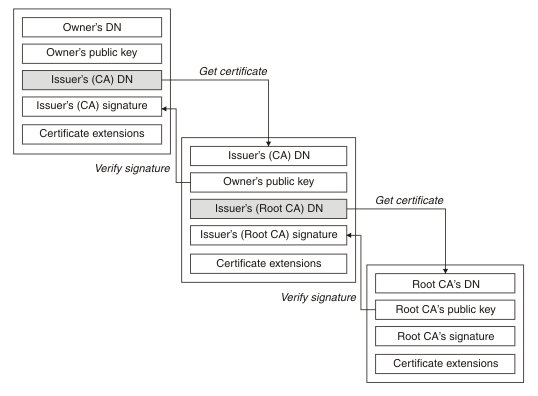
\includegraphics[width=\textwidth]{imgs/certificate_authority_chain.png}
    \caption{Certificate Authority Chain (Source: \href{https://www.ibm.com/docs/en/ibm-mq/8.0?topic=certificates-how-certificate-chains-work}{www.ibm.com/docs})}
    \label{fig:results}
\end{figure}


\end{problems}
\end{document}